\section{Results and Discussion} \label{results}

\subsection{Performance}\label{performance}
The temporal dynamic of a molecular system can be described by the \gls{cme} \todo{REF for CME}.
\gls{gssa}\cite{gillespie_general_1976} produces individual realisations of the \gls{cme}.
In order to obtain accurate estimates of the average dynamic within a population of cell, it is however necessary to perform multiple (often more than $10^4$) simulations.
Despite recent effort \cite{niemi_efficient_2011,dittamo_optimized_2009,komarov_accelerating_2012} to provide fast implementation of this algorithm, computation remains extremely expensive.
This is critical when performing, for instance, parameter inference.
This limitation led to the development of approximations such as \gls{lna}\cite{komorowski_bayesian_2009} and \gls{mea}\cite{ale_general_2013} which can perform in a more reasonable time.

Since the only advantage of \gls{mea} over \gls{gssa} is computational speed, it was paramount to provide an efficient an implementation of \gls{mea}.
In this section, we show that symbolic computations can be limiting for \gls{mea}.
Then, we explain how we have optimised them, and finally increase performance by several order of magnitudes over to the original \mat{} implementation.
In addition, ...\\
\todo{@SL short intro about why it is importan to make solver fast}


\subsubsection{Symbolic expressions}


\gls{mea} involves derivation of a system \gls{ode}s from a model.
This procedure\cite{ale_general_2013}, involves lengthy symbolic calculations.
Even for very simple models (\eg{} three species, five reactions), they cannot be realised manually.
The number $n$ of modelled moments (\ie{} the number of generated \gls{ode}s), for a system with $s$ species and up to moments of order $o$ is defined by:\\
\begin{equation}
n={{s+o-2} \choose {s}} -1
\end{equation}
As a consequence, the complexity of the calculation is predicted to increase exponentially with the number of species in the system and the maximal order of moments.

In order to perform symbolic computations, we have used \sympy{} \cite{sympy_development_team_sympy:_2014}; an efficient \py{} library.
After implementation of the different features (\todo{see section closure/...})
, we have endavoured to optimise the processing speed.
In a first place, we identified significant bottlenecks using \py{} profiling tools.
Then, we designed specific ways to improve speed incrementally without changing the resulting \gls{ode}s.

Figure~\ref{fig:mea_speed} shows the cumulative effects of different optimisations.


\begin{figure}

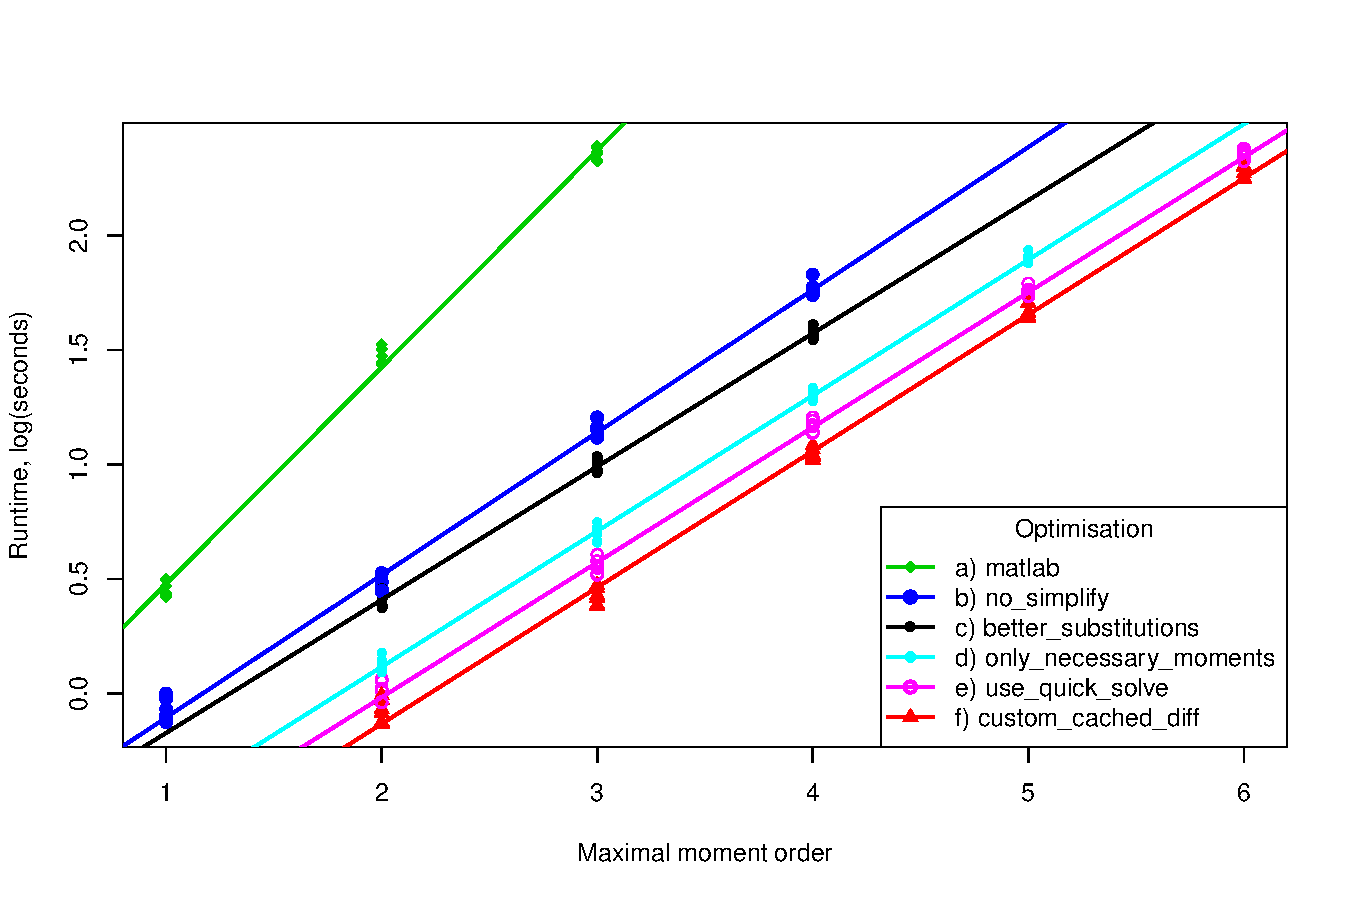
\includegraphics[width=1.0\textwidth{}]{../figure_mea_speed/mea_speed.pdf}
\caption{\emph{Cumulative performance improvement of symbolic calculations resulting from optimisation}.
The processing time for computing log-normal closure on \pft{} model with different maximal moment orders were meseared for original matlab implementation (a) and different optimisations (b$-$f).
In a first place, the calls to \texttt{sympy.simplify()} where removed (b). 
Then, \texttt{sympy.xreplace()} was used instead of \texttt{sympy.substitute()} (c). 
Generating an $(n-s) \times (n_2-s + 1)$ matrix (d), as opposed to an $(n-s) \times (n-s + 1)$ one, also increase speed (see main text).
Implementing a simplified equation solver instead of using \texttt{sympy.solve()} also resulted in a significant speed-up (e). Finally, caching (memoization) \texttt{sympy.diff()} allowed even better performance.
The time complexity appears exponential ($2^{O(n)}$, where $n$ is the maximal moments order) in every case, 
Interestingly, the slopes between, a ($0.95$) and c ($0.58$), and b ($0.62$) and c were significantly different ($p-value <10^{-15}$ and $p-value = 3 \times 10^{-4}$, respectively; t-test on the slopes of the linear regression). 
No significant difference was found between the slopes of the subsequent optimisations (c$-$f). 
However, the intercepts were significantly smaller between each consecutive optimisations after c) ($p-value < 10^{-6}$ for all; t-test on the intercepts of the linear regression).
Nine replicates were performed on the same CPU. For optimisation c$-$f, values corresponding to maximal order moments lower than two were removed because of the inherent inaccuraty in measuring very short durations}
\label{fig:mea_speed}
\end{figure}


The first step involved removing the expression simplification heuristic.
In the original code\footnote{both from the publication and last year's MSc project}, the right-hand-side equations were simplified in order to produce shorter text file results.
However, this was slow and did not benefit subsequent simulations and inference.
For large expressions, simplification had also had an large memory footprint and was likely to fail.
This optimisation significantly improved the scalability of the method (see fig.~\ref{fig:mea_speed}, b).

The next bottleneck was the choice of substitution functions.
As a part of \gls{mea}, it is necessary to replace raw moment symbols by expressions depending on central moments.
Performing substitution can be done using the \texttt{substitute()} function from \sympy, but this is designed to substitute expressions by other expressions.
In most cases, we only had to substitute atomic symbols by expression.
For this purpose, the  \texttt{xreplace()} function was a much more appropriate alternative which resulted in a better scalability (see fig.~\ref{fig:mea_speed}, c).

In the original implementation, a matrix of central moment expression of size $(n-s) \times (n-s + 1)$ is directly generated when the default closure is applied.
However, when using a parametric closure, a matrix of size $(n_2-s) \times (n_2-s + 1)$, where $n_2={{s+o-2 \mathbf{+1}} \choose {s}} -1$, was generated.
The $n_2 - n$ rows corresponding to higher-order moments have then to be deleted.
In contrast, out implementation generates a $(n-s) \times (n_2-s + 1)$ matrix regardless of the closure method.
In addition to improve code readability, consistency and flexibility \footnote{see QG's individual report}, this improved overall performance (fig.~\ref{fig:mea_speed}, d) for cases where closure is applied while keeping the default closure computation fast.

Another simple way to improve computation time was to remove calls to the function \texttt{solve()} which was only used in straightforward cases (\eg{} solving: $a + 2b = c$ for $a$).
It was therefore much more efficient (fig.~\ref{fig:mea_speed}, e) to use simple arithmetic to find solution.

Finally, partial derivation of expression over several variables and order is extensively performed during the approximation.
Generally, these type of differentiations can be simplified several differentiation of first order:
\begin{equation}
\frac{\partial{} ^ 2 f(x,y)}{\partial x \partial y}  =
\frac{\partial{} \frac{\partial{} f(x,y)}{\partial x}}{\partial y} =
\frac{\partial{} \frac{\partial{} f(x,y)}{\partial{} y}}{\partial{} x}
\end{equation}
One advantage, is that, when needing to calculate two derivatives such as:  $\frac{\partial{} ^ 2 f(x,y)}{\partial{} x \partial{} y}$ and $\frac{\partial{} ^ 2 f(x,y)}{\partial{} x^2}$, 
one can precompute $\frac{\partial{} f(x,y)}{\partial{} x}$ and use it for both calculation.
In our implementation, we have use a procedure known as \emph{memoization} which, briefly, permits to store the results of a function call in an associative array.
Then, the next time this function is called with the same arguments, it will return the stored results instead of recomputing it.
This also resulted in an overall perfomance improvement (fig.~\ref{fig:mea_speed}, f).

Reorganising, profiling and rewriting the code resulted in incremental significant performance improvements of symbolic computations in \means{} compared to the original \mat{} code.
For instance, with the same \pft{} system and closure method, 
we predict that computation up to \gls{ode}s up $8^{th}$ order will take 44 minutes with \means{} and as much as 128 days with the original implementation.
This improvement will hopefully contribute to make \gls{mea} realistically usable for systems with more species and reactions

\subsection{Moment Expansion Closure}
Ale \emph{et al.} predicted that increasing the maximal moment order would necessarily result in better approximation \cite{ale_general_2013}.
In addition, preliminary work \todo{cite Eszter,unpublished} indicated that using a parametric distributions for \gls{mea} 
closure could greatly improve approximation. 

The dramatic increase in performance compared to the original code as well as the implementation of parametric closures made it possible to verify these claims.
Figure~\ref{fig:max_order_and_closure_on_distance} shows the effect of increasing maximal moment order and different type of closures.
The \pft system with the originally studied parameters  \cite{ale_general_2013} was used.

For normal and scalar closures, the approximation globally improves with maximal moment order (reduced distance to \gls{gssa}). 
However, for 7$~{th}$ order, the scalar closure had an increased distance, and solving normal closures \gls{ode}s was not possible.
Note that for even maximal moment orders, normal and scalar are rigourously equal.
This is expected because normal distribution is symetrical, thus odd central moments are always zero.

In contrast, log$-$nomal closures are fitting to the ground through trajectory well for maximal moment order of three, 
but the approximation gets less and less accurate for closure at higher and higher order moments.
A closer look at the trajectories indicate that, in this latter case,
oscilations are damping too quickly (fig.~\ref{fig:max_order_and_closure_on_distance}b).
Interestingly for even maximum moment order log$-$normal closures generated \gls{ode}s which,
despide our effort, could not be numerically solved.

For this system and parameter set, univariate and multivariate distributions closures were very similar.





\begin{figure}

\includegraphics[width=1.0\textwidth]{../pipeline/task-output/FigureP53Summary/FigureP53Summary-pdf-7.pdf}
\includegraphics[width=1.0\textwidth]{../pipeline/task-output/FigureP53Simple/FigureP53Simple-pdf-7.pdf}

\caption{\emph{Effect of different closure methods and maximal moment order on simulation accuracy}
The \pft system was modeled using \gls{mea} with five types of closure and for maximal moment order up to seven.
Resulting trajectories were all compared to an average of 5000 \gls{gssa} simulations using sum of square distance (a).
Distance is in log scale.
For illustration puroses, complete trajectories of a single species (\pft) for max order three and seven are shown (b).
Black lines inducate the average of \gls{gssa} simulations. Missing points (b) and lines (a) indicate solver failure 
TODO(see failure section.)


}

 
\label{fig:max_order_and_closure_on_distance}
\end{figure}
